% PKUMpLtX --- A LaTeX document class for 'Modern Physics Laboratory' in PKU based on `revtex4-2`
%
% Please read `README.md' and the template file before using
% 需要确保 font 选项指定的字体已安装! 具体参见 `README.md' 的说明.
\documentclass[font=default]{mpltx}

% 以下至 \begin{document} 都仅是本文件为了方便额外定义的命令, 写报告时不需要.
\hypersetup{colorlinks=true}% 超链接带颜色
\usepackage{xcolor}
\usepackage{tcolorbox}

\newtcbox{\buttombox}[1][red]
  {on line, arc = 3pt, outer arc = 3pt,
    colback = #1!10!white, colframe = #1!50!black,
    boxsep = 0pt, left = 2pt, right = 2pt, top = 1pt, bottom = 1pt,
    boxrule = 1pt}

\newcommand{\note}[1]{{\color{gray}#1}}
\NewDocumentCommand{\pkg}{s o m}{%
    \IfBooleanF{#1}{%
        \IfNoValueTF{#2}%
            {\href{https://www.ctan.org/pkg/#3}}%
            {\href{https://www.ctan.org/pkg/#2}}%
    }%
    {\textsf{#3}}%
}
\newcommand*\cs[1]{\texttt{\textbackslash #1}}
\newcommand*\env[1]{\textit{\texttt{#1}}}
\newcommand*\code[1]{\texttt{#1}}
\newcommand*\file[1]{\textbf{\texttt{#1}}}
\makeatletter
\newcommand\releasedate{%
    \href{https://github.com/CastleStar14654/PKUMpLtX/releases/tag/\mpltx@fileversion}%
        {\mpltx@filedate, \mpltx@fileversion}}
\makeatother
% 以上是本文件为了方便额外定义的命令, 写报告时不需要.

\begin{document}

\title{声光调制锁模激光器} % 切合报告内容, 简短明确, 可以不同于讲义
\author{罗俊熙} % 这里 \emailphone 一定要紧跟在 \author 后方
\emailphone{see.looooo@stu.pku.edu.cn}{(86)13611162432}
% 如果改用 \email 则仅需要邮箱参数
\affiliation{北京大学物理学院\quad 学号: 2000012508}
% % 可以使用 \zhdate 自动生成中文日期, 如
% \date{\zhdate{2020/12/1}}
% % 也可使用 babel 的 \localedate, 如
% \date{\localedate{2020}{12}{1}}
% % 两者均会输出 `2020 年 12 月 1 日'
% 下面的 \date 的参数是为了自动输出正确版本号, 正式报告请替换为上面的两种 \date 之一
\date{\localedate{2023}{03}{04}}
\begin{abstract}
	短脉冲光源被应用在非线性光学、激光光谱学等。激光器的锁模技术在80年代后成为强短脉冲激光的产生方法,而锁模的方法又分主动和被动两种,
    这次实验将使用声光调制的方法,对激光进行主动锁模调制。观察拉曼-奈斯(Raman-Nath)衍射现象,
    并测出0级衍射光束的衍射效率与电功率关系,并通过调节产生锁模激光源。
\end{abstract}
\keywords{声光调制, 锁模激光, 拉曼-奈斯衍射}

\maketitle

\section{引言}
激光器是现代物理中经常使用的光源,其单色性、强度以及一些量子特性令其能广泛地应用在许多科研场境。而在激光器共振腔内的光能在两面反射镜之间产生驻波,不同频率的驻波形成了激光的模式。
一般的激光器中,这些模式都是相互独立的、没有关系的。各模式间的相位亦无固定的关系,这些模式的相互叠合,能产生许多有用的物理现象,比如只有几个振荡模式的激光哭中,
模式之间可能出现拍频的现象,令激光强度产生随机波动。\par

如果将这些模式间的相位固定,激光器就会产生一个全新的工作模式—锁模激光。这种激光会周期性地输出一个强而又窄的光脉冲。脉冲的长度通常在皮秒($10^{-12}$)到飞秒($10^{-15}$)的级别。
这能够应用在许多测量计术上,尤其提供了一个很好的途径研究非线性光学。\par

本实验是在 He-Ne 激光器中的腔内插入声光损耗调制器来进行主动调制,用以实现对$\qty{633}{\nm}$激光的锁模。并通过这次实验,学习和掌握激光锁模和声光调制的原理;
掌握锁模激光器结构特点和调试方式;观察腔长的变化及调制深度对于输出的光脉冲的影响。

\section{理论}\label{sec:theory}
\subsection{锁模激光器}
激光输出的条件是光在谐振腔内多次往返传播中式稳定持续的驻波,即光在谐振腔往返一周的光程为波长的整数倍:
$$2L=q\lambda_q$$
其中,腔长为$L$,$q$为纵模序数,$\lambda_q$为波长。由于$q$被限制为整数,因此每个$q$对应着一种稳定的电磁场分布模式,而不同纵模对应的圆频率为:
$$\omega_q=2\pi\nu_q=q\frac{2\pi c}{2L}$$
相领从模的频率差为:
$$\Delta \omega= 2\pi \Delta \nu = \frac{\pi c}{L}$$
若激光介介质增益线宽为$\omega_G$,则激光腔内会有$N=\frac{\omega_G}{\omega}$个纵模出现。\par

如上所述,这些纵模是相互独立地存在的,他们的相位$\varphi_q$间是随机变化的,激光的输出强度近乎为一个常数。但若令每个纵模的相位有固定的联系,或所有纵模的相位都一样,则他们会在激光腔内发生相干叠加。
比如说令$\varphi_q=0$,能量$E_p=E_0$时,总输出的光强应为:
$$I(z,t)=|E(z,t)|^2=E_0^2\times\frac{\sin^2(\frac{1}{2}N\Delta\omega\cdot(t-\frac{z}{c}))}{\sin^2(\frac{1}{2}\Delta\omega\cdot(t-\frac{z}{c}))}$$
可以看出,光强是一个行进的波包。\par

这次实验采用的是主动锁模的调幅技术,在泪光腔内插入损耗调制器,使激光内部的纵模能够收到周期性的损耗调制信号,使其锁模。
一般来说我们可以假定损耗调制的函数形式为:
$$\delta=\delta_0\cos(\Delta\omega_Mt)$$
其中$\Delta\omega_M$为调制频率(这里不限于这种函数形式,只要是基频为$\Delta \omega_M$的周期性函数即可),受到损耗调制的第$q$个纵模振动为:
$$E_q(t) =  E_{q}(\omega_q) + \frac{1}{2}\delta_0 E_{q}(\omega_q+\Delta\omega_M) +\frac{1}{2}\delta_0E_{q}(\omega_q-\Delta\omega_M)$$
其中$E_{q}(\omega)=E_{0q}\times\cos{(\omega t + \varphi_q)}$。因此就会形成频率为$\omega_q,\omega_{q+},\omega_{q-}$三种频率的振动。当$\Delta\omega_M=\Delta\omega$的时侯,
边频频率正好与$\omega_{q\pm1}$相耦合,这些耦合的纵模又会继续和调制源继续相互作用,最后令增益线宽内所有纵模都会耦合,实现同步振动,达到激光的锁模。

\subsection{声光调制}
本次实验中,将使用声光调制的方法对激光进行锁模,而所使用的声光介质则为熔石英,折射率为$n=1.457$,这种物质能产生声光效应,即当介质有超声波传播时,超声波使波导介质产生应变,
因而使介质的折射率出现少许变化,光通过这种介质就像通过一个厚光栅,能产生衍射、偏转、频移及强度的变化。比如说,在芋一时刻观测声光效应,光就会因这种厚光栅的作用,根据入射角
的不同和声光相互作用区的长短不同,产生拉曼-奈斯(Raman-Nath)衍射和布拉格(Bragg)衍射。要在 He-Ne 激光器中实现声光器件的损耗调制,必须要将衍射损耗控制在 $10\%$ 以内,
以达到光的放大加强。只要入射光与衍射光速方向一致,拉曼-奈斯衍射中的0级衍射性能就能实现此效果。


\section{实验装置及流程}
\subsection{实验装置}
包括 He-Ne 激光器、声光调制器、激光电源、布儒特斯窗片及反光镜等。实验光路如\autoref{fig:1}所示:

\begin{figure}
    \centering
    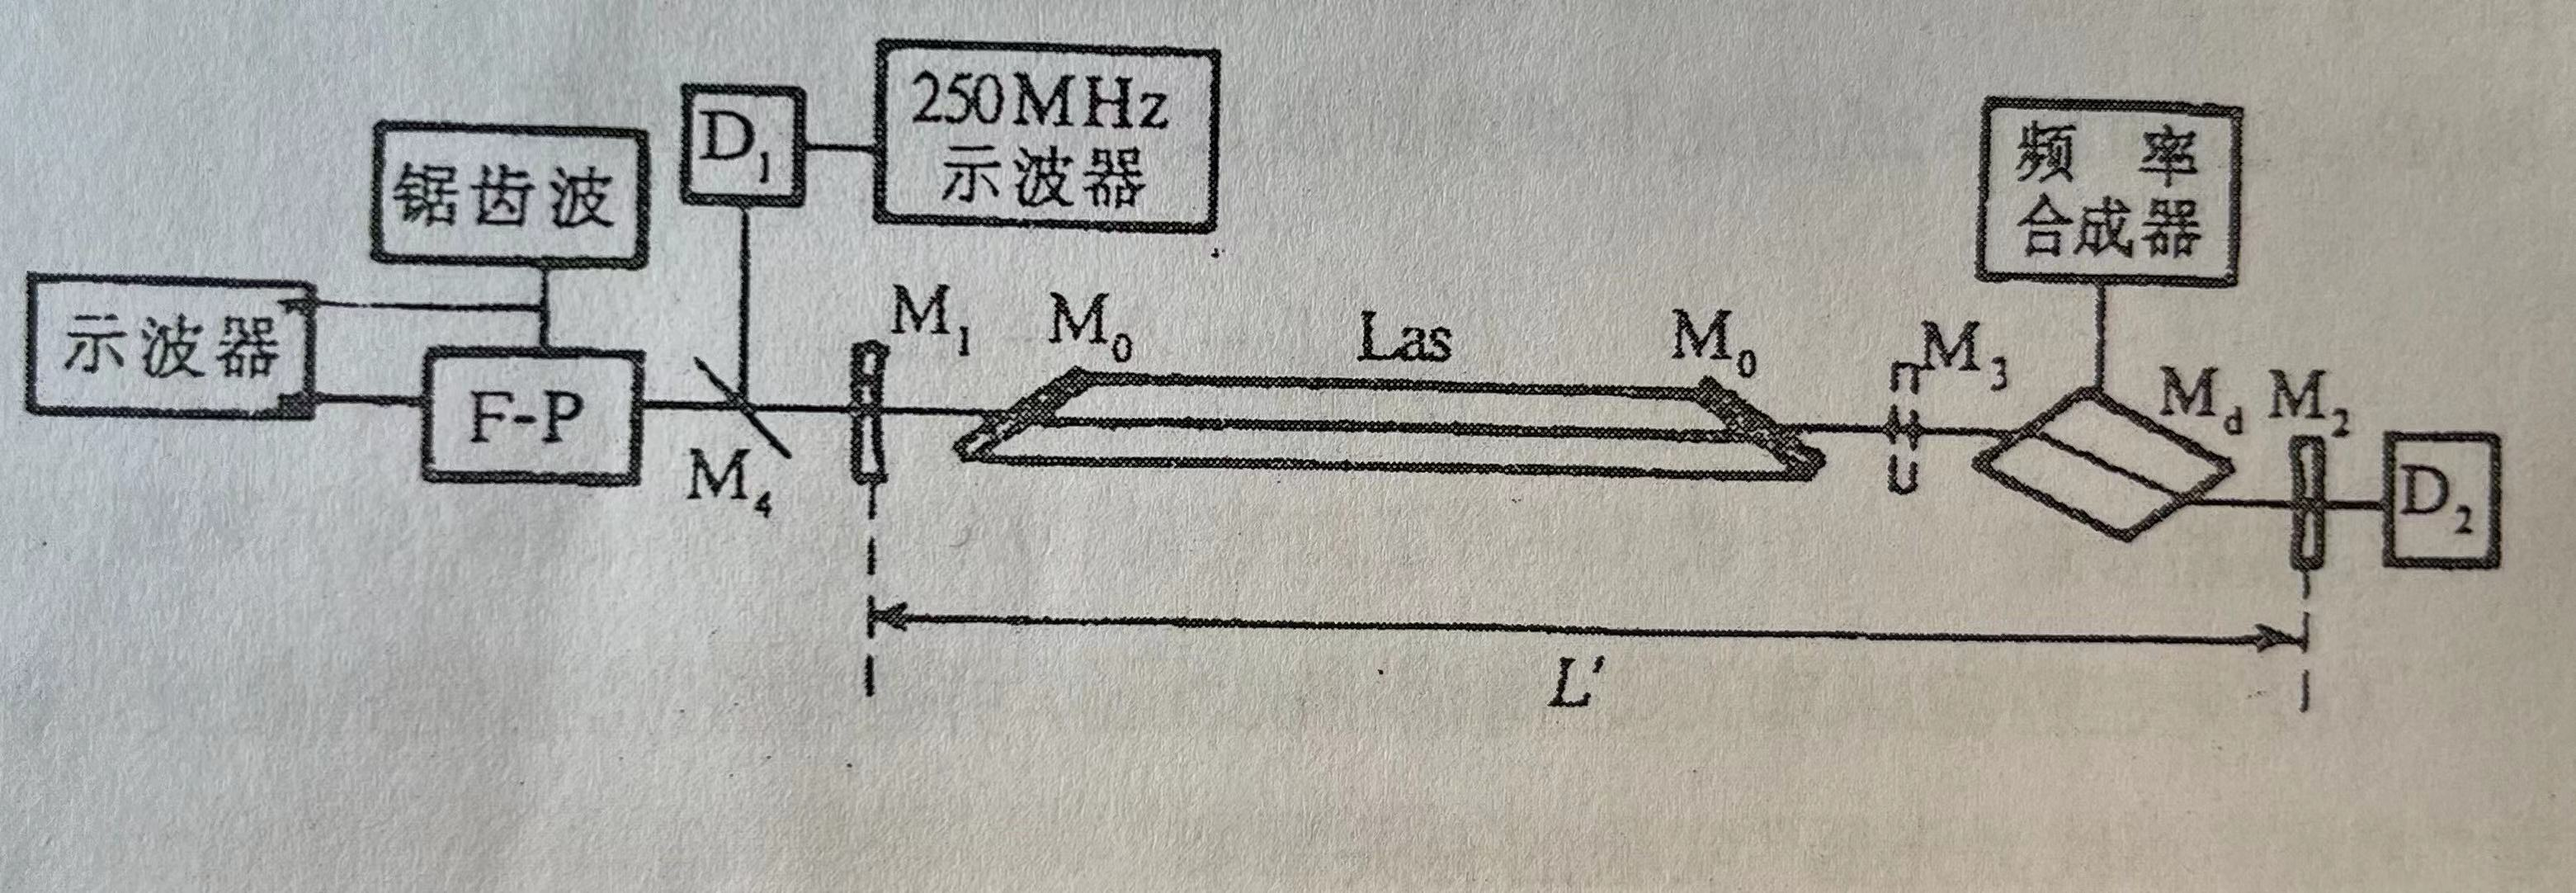
\includegraphics[width=0.85\linewidth]{fig/1.jpg}
    \caption{实验光路图\cite{laser}}
    \label{fig:1}
\end{figure}

\subsection{实验过程及结果}
连接电路,调整光路,点燃激光器。\note{如果可以的话,在这里使用扫描干涉仪观察激光器的输出纵模频谱,并记录当中的:纵模个数、强度和稳定性等。}\par
调整超声频率,使得激光光强最大,衍射级数多而对称。如\autoref{fig:2}所示,这时超声波的角频率为$\Omega=\qty{285.8}{\MHz}$,其对应的频率为$f=\frac{\Omega}{2\pi}=\qty{45.48}{\MHz}$。

\begin{figure}
    \centering
    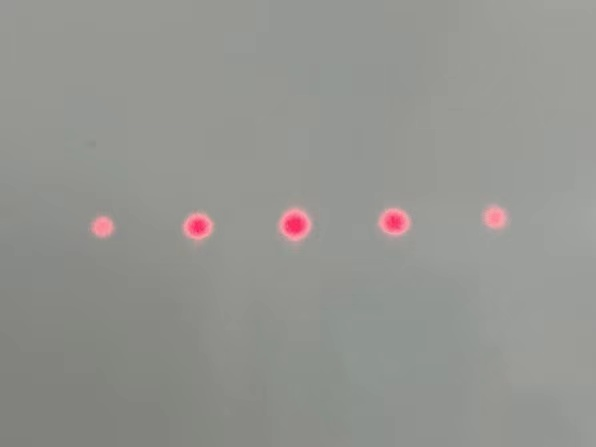
\includegraphics[width=0.45\linewidth]{fig/2.jpg}
    \caption{声光介质致的拉曼-奈斯效应,在极大两侧分别有两个次极大。}
    \label{fig:2}
\end{figure}

计算激光腔的实际几何长度$L'$:声光介质材料用的熔石英折射率为$n=1.457$,长度为$l=\qty{17}{\mm}$,厚度为$d=\qty{2}{\mm}$,为减少可能产生的插入损耗,声光介质的入射和出射界面为布儒斯特角:
$$\theta_b=\arctan{\frac{1}{n}=\qty{34.46}{\degree}}$$
根据调制器的角频率$\Omega$,可以得到激光器所需的光程长度为:
$$L=\frac{\pi c}{2\Omega}=\qty{1647.9}{\mm}$$
调制器的和激光管的窗片的光程和几何程差分别为:
$$\begin{aligned}
	\Delta_1 &= nl-l\sin{(2\theta_b)}=\qty{8.91}{\mm} \\
	\Delta_2 &= \frac{nd}{\cos{\theta_b}}-\frac{d\cos{(2\theta_b)}}{\cos{(\theta_b)}} = \qty{2.66}{\mm}	
\end{aligned}$$
我们可以得到激光腔的实际几何长度应为:
$$L'=L-\Delta_1-\Delta_2=\qty{1636.4}{\mm}$$
在实验台上,反光镜$M_1$被放置在$x=\qty{12}{\cm}$处,因此$M_2$应放在$x'= \qty{1756.3}{\mm}$处的位置。\par
在$M_1$、$M_3$下调制$M_2$位置和角度,使得激光光强最大化,取下$M_3$后继续微调$M_2$,那么激光就能实现振荡放大的效果,但并没有成功调节出激光,因此实验在这里中止了。

% 放上声光调制器于$M_2$前,放回$M_3$,调出激光后,取下$M_3$,此时通过校准,调制出锁模激光。
% 通过$D_1$测量找出脉冲周期$T_e$和脉冲宽度$\Delta l_e$,理论计算得到脉冲周期$T_t=$和脉冲宽度为$\Delta l_t=$,
% \note{这里推测应该理论值要少一些,因为脉冲波包会发生群速度色散,使波宽展开。}

% 将激光通入扫描干涉仪观察激光的纵模频谱,并与没锁模状态下的激光作比较。\par

% 改变声光调制器上的输入电功率,观察其对锁模状态的影响,找出最佳锁模电功率和相应的声功率和零级衍射调制度。

\section{结论}
\textbf{本次实验利用实验至提供的 He-Ne 激光器,成功通过声光损耗调制器调节出现拉曼-奈斯衍射。
并尝试调节激光器使得其能通过声光损耗调制器产生共振,不过并没有成功。}

% bibliography 的参数是你的 *.bib 文件去掉后缀名后的部分
\bibliography{bibli}

\clearpage % 附录前另起一页
\appendix % 附录开始
\section{思考题}\label{app:exercise}
\subsection{为甚么实验失败?}
实验中失败的原因有很多,其中一个我认为一激光的起振条件是光路长度为波长的整数倍,因此调节上极为困难,而且实验中的光路也没有很好的尺标和导轨,在实验中的额外自由度让我们十分困扰。最后是调节反射时并没有很好的方法,我们小组决定是将输出的像和反射后输出的像尽量重合,这可能和实际有一些出入。
\subsection{锁模用的声光调制哭能用行波的方式工作吗?为甚么?}
应该是不可以的,因为声光衍射是利用驻波在不同地方产生的不同弹性形变来产生折射率的变光,产生拉曼—奈斯效应。若以行波的方式工作,那么声光介质的工作模式会异常地复杂,而且衍射光极有可能是关于时间$t$的函数,不利于实验的进行。
\subsection{为甚么要把声光调制器安放在尽量靠近谐振腔反射镜的一端?}
在计算时,可以认为激光器的转出是间隔为$2\frac{L}{C}$的固定周期性序列,也就是光在腔内往返一次的时间,因此把声光调制器放在靠近谐振腔反射镜的一端能够减少$L$的误差。
\subsection{请设计一个准确测量锁模脉宽的方案。}
使用类似迈克尔逊干涉仪的设计,将一半的输出通过半反镜转移到另一光路上,一光臂接上能探测峰值的仪器,另一边则放上反射镜,仔细调整就能类似根据两个艾瑞班的叠加来判定半波全宽是多少了。

\end{document}
